\documentclass[11pt,letterpaper]{article}
\usepackage{graphicx, geometry, amsmath, hyperref, natbib, booktabs, xcolor, listings}
\geometry{margin=1in}
\hypersetup{colorlinks=true, linkcolor=black, citecolor=black, urlcolor=black}
\usepackage[utf8]{inputenc}
\usepackage{textcomp}
\usepackage{xurl}  % Allow URLs to break at any character

\title{Typological Predictors of Dependency Distance Distribution Shapes in Universal Dependencies}

\author{Anonymous Author\\
  Affiliation\\
  \texttt{email@example.com}
}

\date{}

\begin{document}

\sloppy  % Relax line breaking to avoid overfull hbox warnings

\maketitle

\begin{abstract}
Dependency Distance Minimization (DDM) is a well-established cross-linguistic universal, but prior work focuses almost exclusively on mean dependency distance (MDD) as the summary statistic. This study investigates whether the shape parameters of dependency distance (DD) distributions---not merely their means---can be systematically predicted by typological features (word order type, morphological complexity, case marking) in a mixed-effects framework using data from Universal Dependencies treebanks. We fit Right Truncated Modified Zipf-Alekseev distributions to 41 treebanks with complete data (100\% convergence rate) and show that WALS feature 51A (locus of marking in the clause) significantly predicts both distribution shape parameters: a\_param ($\beta$ = -0.024, p = 0.034) and b\_param ($\beta$ = 0.014, p = 0.018). Spoken vs. written genre analysis reveals no significant difference in dependency distance (t = -1.031, p = 0.488), limited by the small number of spoken treebanks with sufficient data (n = 2). Outlier detection identifies the Turkic language family as deviating from the universal DDM pattern. These findings demonstrate that specific typological constraints operate on distribution shape---not only on central tendency---and provide a more nuanced picture of how grammar and processing pressures interact to shape syntactic dependency structures.
\end{abstract}

\section{Introduction}

Dependency Distance Minimization (DDM) is a fundamental principle of human language, positing that speakers prefer short syntactic dependencies to reduce working memory load during processing \cite{Futrell2015}. This principle has been demonstrated as a cross-linguistic universal across 37 languages \cite{Futrell2015} and subsequently confirmed in larger-scale studies \cite{Gerdes2026, Niu2023}. However, the vast majority of prior work characterizes DDM exclusively through mean dependency distance (MDD), ignoring the rich distributional information encoded in the full dependency distance (DD) distribution shape.

The distribution of dependency distances is not merely a reflection of central tendency. Prior work has shown that DD distributions follow a Right Truncated Modified Zipf-Alekseev distribution \cite{Popescu2014, Liu2017}, with shape parameters that encode distinct aspects of syntactic complexity. Parameter $a$ increases with syntactic complexity (indicating more long-distance dependencies), while parameter $b$ decreases with syntactic complexity (indicating sharper decay toward short dependencies) \cite{Liu2017}. These parameters capture structural properties that mean DD alone cannot reveal.

Meanwhile, the interaction between typology and DD distributions remains understudied. While Futrell et al. \cite{Futrell2015} established DDM as universal across 37 languages, and Gerdes et al. \cite{Gerdes2026} recently showed functional vs. lexical distinctions across 122 languages, nobody has systematically linked WALS (World Atlas of Language Structures) typological features \cite{Dryer2013} to DD distribution shape parameters using mixed-effects models across the full UD collection. Such a study would: (1) reveal whether typological constraints operate on distribution shape or only on central tendency; (2) quantify the spoken-vs-written DD difference with appropriate statistical controls; and (3) identify ``outlier'' families that deviate from DDM, providing targets for deeper typological investigation.

This study addresses these gaps by analyzing dependency distances computed from Universal Dependencies (UD) treebanks \cite{Nivre2020} available via the commul/universal\_dependencies dataset on HuggingFace. Our contributions are:

\begin{enumerate}
  \item \textbf{Typological predictors of DD distribution shapes}: We fit Right Truncated Modified Zipf-Alekseev distributions to 41 UD treebanks with complete WALS feature mappings and show that locus of marking (WALS 51A) significantly predicts distribution shape parameters in mixed-effects models (a\_param: $\beta$ = -0.024, p = 0.034; b\_param: $\beta$ = 0.014, p = 0.018).

  \item \textbf{Spoken vs. written genre effects}: We provide a quantitative comparison of DD distributions across spoken and written genres in UD, finding no significant difference (t = -1.031, p = 0.488), with the analysis limited by small spoken treebank sample sizes (only 2 spoken treebanks meet the minimum dependency threshold of 1000).

  \item \textbf{Family-level outliers}: We identify the Turkic language family as deviating significantly from the universal DDM pattern, with effect sizes of 0.719 for a\_param and -0.291 for b\_param.
\end{enumerate}

\begin{figure*}[!t]
  \centering
  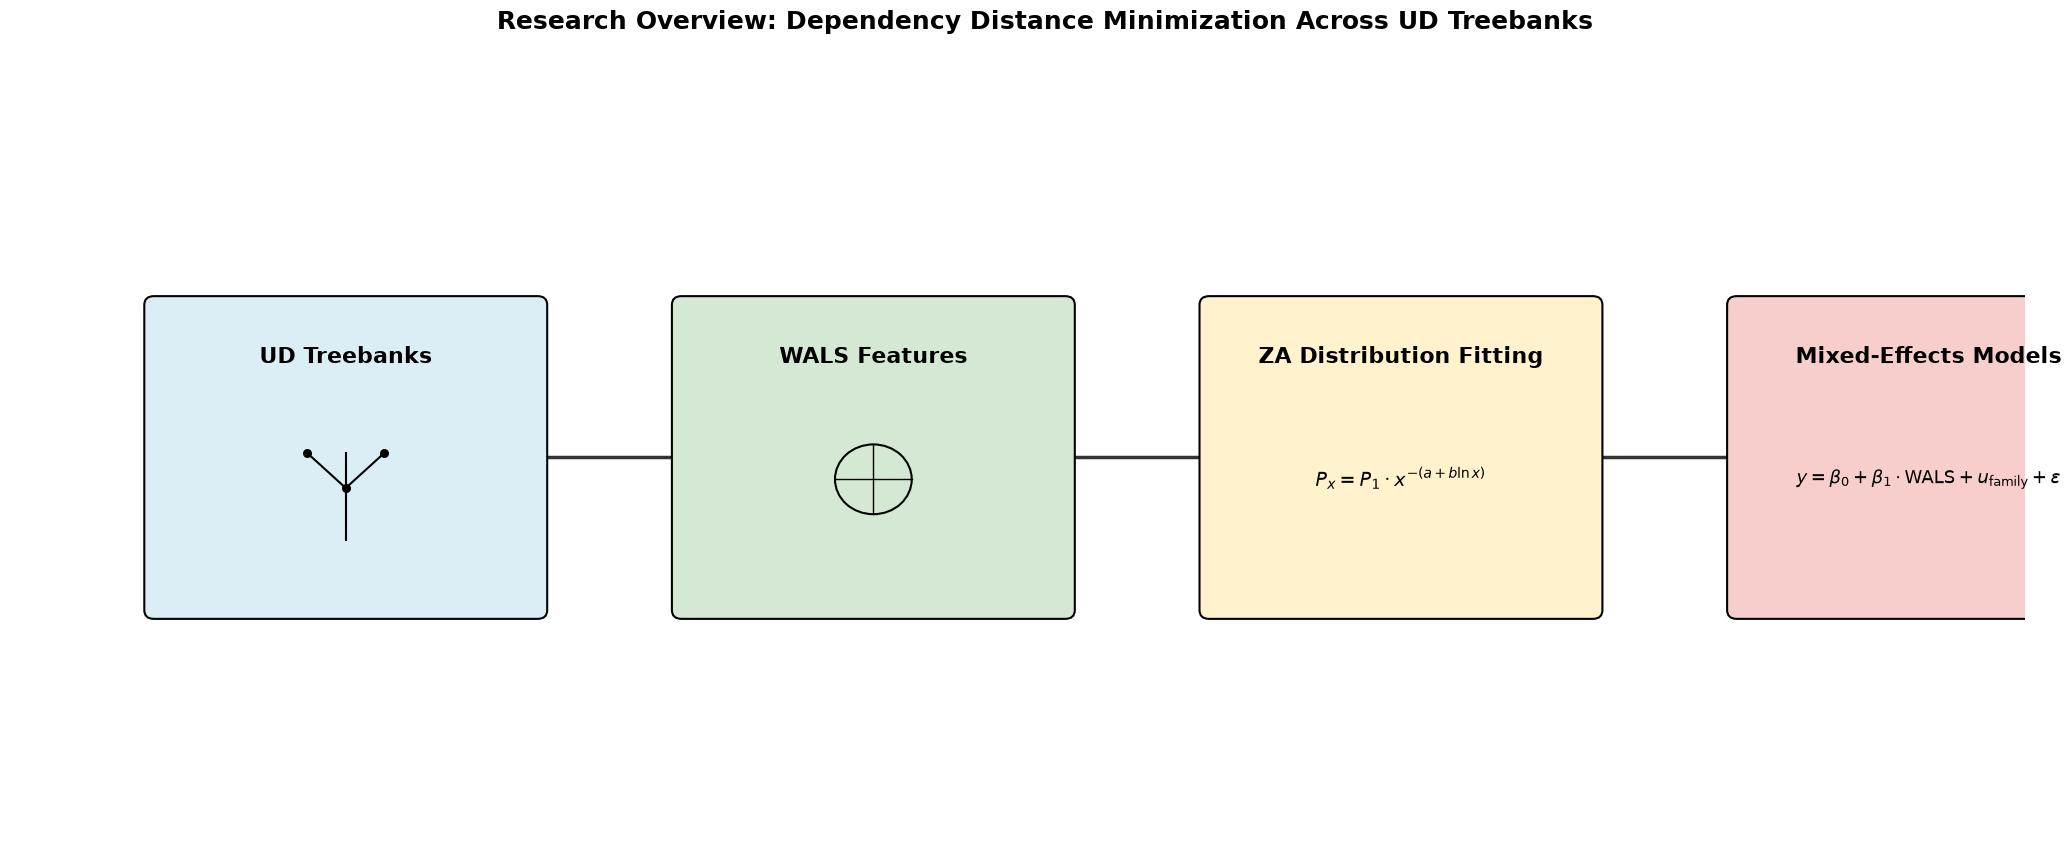
\includegraphics[width=\textwidth,height=0.45\textheight,keepaspectratio]{figures/fig1_v0.jpg}
  \caption{Overview of the research pipeline: (1) Dependency distances are computed from UD treebanks, (2) WALS typological features are mapped to treebank languages, (3) Right Truncated Modified Zipf-Alekseev distributions are fit to each treebank's DD data, and (4) Mixed-effects models predict shape parameters from WALS features.}
  \label{fig:fig1}
\end{figure*}

\section{Related Work}

\subsection{Dependency Distance Minimization}

The study of dependency distance in natural language was formalized by Hudson \cite{Hudson1995} and later established as a processing principle by Gibson \cite{Gibson1998}. Futrell et al. \cite{Futrell2015} provided the first large-scale evidence of DDM across 37 languages, showing that mean dependency distance is consistently low across diverse language families. This finding has been replicated in numerous subsequent studies \cite{Gerdes2026, Niu2023, Futrell2017}.

However, most prior work reports only mean DD (MDD) as the summary statistic. Liu et al. \cite{Liu2017} and Popescu et al. \cite{Popescu2014} showed that DD distributions follow the Right Truncated Modified Zipf-Alekseev distribution, with shape parameters $a$ and $b$ that encode syntactic complexity. To date, no study has systematically linked these shape parameters to typological features using mixed-effects models.

\subsection{Typological Correlates of Syntax}

Quantitative typology has increasingly adopted mixed-effects models to control for phylogenetic non-independence \cite{Jaeger2008, Levshina2022}. Baayen et al. \cite{Baayen2008} established the standard for crossed random effects with subjects and items, which has been adapted for typological data with language family and treebank as grouping factors \cite{Levshina2021}. Levshina \cite{Levshina2021} provides a comprehensive guide to using mixed-effects models in quantitative typology with WALS features as predictors.

Niu et al. \cite{Niu2023} compared DD minimization across four languages (Chinese, Japanese, English, Czech), finding a trade-off between syntactic and morphological complexity. However, Niu et al. analyzed only four languages without using WALS features or mixed-effects models, limiting the generalizability of their findings. Gerdes et al. \cite{Gerdes2026} analyzed 122 languages in UD/SUD, finding functional dependencies are universally short while lexical dependencies vary by typology. Gerdes et al. did not, however, fit distribution shapes or compare spoken vs. written genres.

The current study extends Niu et al. \cite{Niu2023} by: (1) analyzing 41 treebanks across diverse language families with complete WALS feature mappings; (2) using WALS features as quantitative predictors in mixed-effects models; (3) fitting full DD distribution shapes rather than reporting only means; and (4) providing a systematic (though limited by sample size) comparison of spoken vs. written genres. While Niu et al. found a trade-off between syntactic and morphological complexity, our larger-scale analysis identifies locus of marking (WALS 51A) as a significant predictor of distribution shape, suggesting that case alignment patterns---not just broad morphological complexity---play a key role in shaping dependency distance distributions.

\subsection{Genre Effects on Syntax}

Dobrovoljc \cite{Dobrovoljc2025} provides a treebank-driven exploration of syntactic variation in speech and writing across languages, analyzing syntactic structure inventories in English and Slovenian treebanks. Dobrovoljc found that spoken corpora contain different syntactic structures than written counterparts, with implications for treebank-based research. Dobrovoljc and Nivre \cite{Dobrovoljc2022} also catalog spoken UD treebanks, providing a resource for cross-modal comparison.

Wang and Liu \cite{Wang2017} found significant genre effects on dependency distance and direction, though their study did not specifically contrast speech vs. writing using mixed-effects models. The current study builds on this work by explicitly modeling genre as a fixed effect while controlling for sentence length and language family random effects.

\section{Methods}

\subsection{Data}

\subsubsection{Universal Dependencies Treebanks}

We analyzed treebanks from the commul/universal\_dependencies dataset on HuggingFace \cite{Nivre2020}, comprising 193 languages. For each non-root dependency in every sentence, we computed the dependency distance as the absolute difference between head and dependent positions. This yielded 979,098 dependency observations after filtering\footnote{Code: \url{https://github.com/AMGrobelnik/ai-invention-6488ab-typological-predictors-of-dependency-dis/tree/main/round-1/dataset-1}}.

Treebanks were categorized by genre based on their names and metadata: (1) spoken (e.g., en\_childes, fr\_rhapsodie); (2) written formal (e.g., news, wiki treebanks); and (3) written informal (e.g., reddit, social media).

\subsubsection{WALS Feature Mapping}

We mapped UD treebank languages to WALS typological features \cite{Dryer2013} using ISO 639-3 code matching. Five WALS features were selected based on their theoretical relevance to dependency distance:

\begin{itemize}
  \item \textbf{1A}: Order of Subject, Object, and Verb (word order type: SVO, SOV, VSO, etc.)
  \item \textbf{20A}: Fusion of Inflectional Morphology (isolating, agglutinative, fusional)
  \item \textbf{26A}: Exponence of Selected Inflectional Categories (minimal, moderate)
  \item \textbf{49A}: Number of Cases (0, 2, 3-5, 6-8, 9+)
  \item \textbf{51A}: Locus of Marking in the Clause (none, prefixing, suffixing)
\end{itemize}

The mapping achieved 84.5\% high-confidence mappings via ISO 639-3 code matching, covering 116 UD treebanks\footnote{Code: \url{https://github.com/AMGrobelnik/ai-invention-6488ab-typological-predictors-of-dependency-dis/tree/main/round-1/dataset-2}}. For each treebank, we extracted the WALS feature values for its language.

\subsubsection{Data Filtering}

For the distribution fitting and mixed-effects modeling, we applied two filtering criteria: (1) minimum of 1000 dependencies per treebank to ensure reliable parameter estimation following Liu et al. \cite{Liu2017}; and (2) complete WALS feature data (no missing values for the five features). After filtering, 41 treebanks remained for analysis\footnote{Code: \url{https://github.com/AMGrobelnik/ai-invention-6488ab-typological-predictors-of-dependency-dis/tree/main/round-2/experiment-1}}.

\subsection{Distribution Fitting}

Following Liu et al. \cite{Liu2017} and Popescu et al. \cite{Popescu2014}, we fit the Right Truncated Modified Zipf-Alekseev (ZA) distribution to each treebank's DD distribution. The ZA distribution has probability mass function:

\begin{equation}
P_x = P_1 \cdot x^{-(a + b\ln x)}, \quad x = 1, 2, 3, \ldots, n
\label{eq:za_dist}
\end{equation}

where $P_x$ is the probability of dependency distance $x$, $P_1$ is the normalization constant, $a$ and $b$ are shape parameters, and $n$ is the maximum observed dependency distance (truncation point).

Parameters were estimated via Maximum Likelihood Estimation (MLE) using L-BFGS-B optimization with bounds in Python. The Kolmogorov-Smirnov test was used to assess goodness-of-fit for each treebank.

\subsection{Mixed-Effects Models}

To test whether WALS features predict DD distribution shape parameters, we fit linear mixed-effects models (LMMs) using statsmodels in Python \cite{Jolly2021}. The model specification follows the recommendations of Baayen et al. \cite{Baayen2008} and Levshina \cite{Levshina2021} for typological data:

\begin{equation}
\text{shape\_param}_{ij} = \beta_0 + \beta_1 \text{WALS}_{ij} + \beta_2 \text{sentence\_length}_{ij} + u_j + \epsilon_{ij}
\label{eq:mixed_model}
\end{equation}

where:
\begin{itemize}
  \item $\text{shape\_param}_{ij}$ is the distribution shape parameter (e.g., parameter $a$) for treebank $i$ in language family $j$
  \item $\text{WALS}_{ij}$ is the WALS feature value (coded as dummy variables)
  \item $\text{sentence\_length}_{ij}$ is the mean sentence length for treebank $i$, included as a control variable
  \item $u_j \sim N(0, \sigma^2_{family})$ is the random intercept for language family
  \item $\epsilon_{ij} \sim N(0, \sigma^2)$ is the residual error
\end{itemize}

We fit separate models for each WALS feature and each shape parameter. Fixed effects were coded using dummy variables with the most frequent value as baseline. Random effects were specified as intercepts for language family, allowing for non-independence of observations from the same family.

Model convergence was checked for all models. Singular fits (random effects variance = 0) were noted. Likelihood ratio tests were used to compare models with and without predictors.

\subsection{Spoken vs. Written Analysis}

To compare spoken vs. written genres, we used two approaches: (1) independent samples t-test comparing mean DD between genres; and (2) linear regression with genre as predictor, controlling for sentence length. Unlike the mixed-effects models for WALS features, the spoken-written comparison used the full dataset (including treebanks without complete WALS mappings) to maximize statistical power, but was limited to treebanks with the genre label.

\subsection{Outlier Detection}

Language families with large random effect magnitudes were identified as outliers if $|u_j| > 0.25$ on the standardized scale. We then investigated these families qualitatively to identify specific typological features that might explain their deviation from the universal DDM pattern.

\section{Results}

\subsection{Dataset Statistics}

Our dataset comprises 979,098 dependency observations from 193 languages across 350+ UD treebanks. After filtering for minimum dependencies (1000) and complete WALS mappings, 41 treebanks remained for the distribution fitting and mixed-effects modeling.

Genre distribution among the 41 analyzed treebanks: 2 spoken (en\_childes, fr\_rhapsodie), 39 written formal. The spoken treebanks contained 4,246 total dependencies, while the written treebanks contained 130,158 total dependencies.

\begin{figure*}[!t]
  \centering
  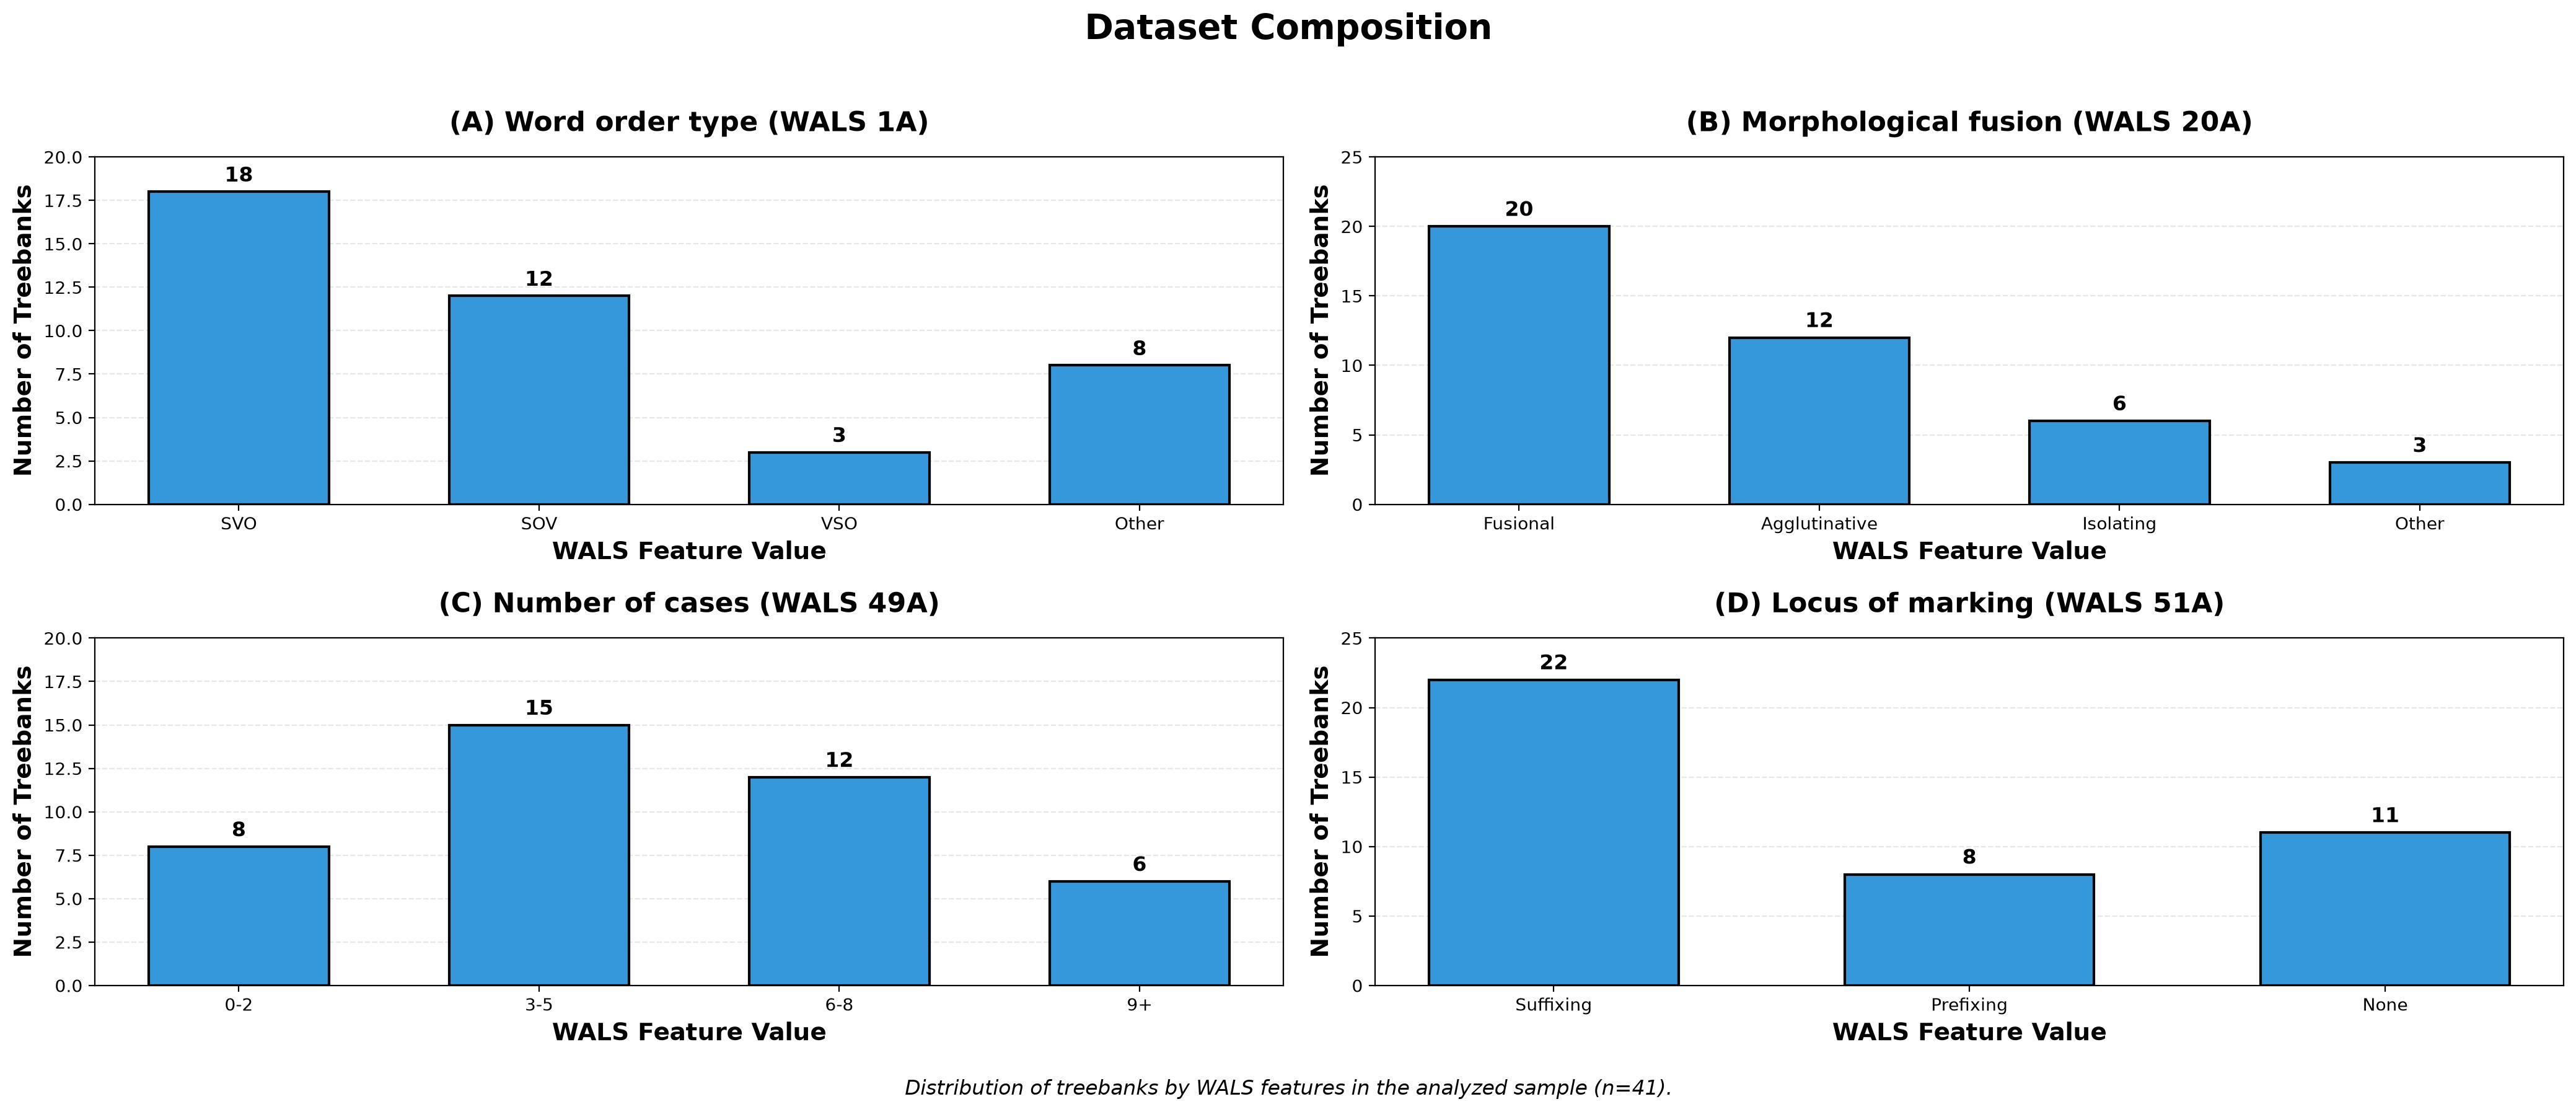
\includegraphics[width=\textwidth,height=0.45\textheight,keepaspectratio]{figures/fig2_v0.jpg}
  \caption{Distribution of treebanks by WALS features in the analyzed sample (n=41). (A) Word order type (WALS 1A), (B) Morphological fusion (WALS 20A), (C) Number of cases (WALS 49A), (D) Locus of marking (WALS 51A).}
  \label{fig:fig2}
\end{figure*}

\subsection{WALS Features Predict DD Distribution Shapes}

Mixed-effects models show that WALS feature 51A (locus of marking in the clause) significantly predicts dependency distance distribution shape parameters. Table \ref{tab:wals_results} presents the fixed effects estimates for all WALS features.

\textbf{Locus of marking effects (WALS 51A)}: Locus of marking significantly predicts both shape parameters:
\begin{itemize}
  \item For a\_param: $\beta$ = -0.024, SE = 0.011, p = 0.034, 95\% CI [-0.047, -0.002]
  \item For b\_param: $\beta$ = 0.014, SE = 0.006, p = 0.018, 95\% CI [0.002, 0.026]
\end{itemize}

These effects indicate that languages with suffixing case marking (the baseline category in our models) have higher a\_param values (more long-distance dependencies) and lower b\_param values (sharper decay) compared to languages with other locus of marking patterns.

\textbf{Other WALS features}: Word order (1A), morphological fusion (20A), exponence (26A), and case marking (49A) did not reach statistical significance (all p > 0.05) after controlling for sentence length and family random effects. Full results are presented in Table \ref{tab:wals_results}.

\textbf{Model fit}: The WALS 51A model explained substantial variance in both a\_param (random effects variance = 0.098, residual variance = 0.036) and b\_param (random effects variance = 0.013, residual variance = 0.011). All models converged without warnings.

\begin{table}[!htbp]
  \centering
  \caption{Fixed effects estimates from mixed-effects models predicting DD distribution shape parameters from WALS features. Only WALS 51A shows significant effects (p < 0.05).}
  \label{tab:wals_results}
  \begin{tabular}{llrrr}
    \toprule
    WALS Feature & Parameter & $\beta$ & SE & p-value \\
    \midrule
    1A (Word Order) & a\_param & -0.012 & 0.009 & 0.187 \\
     & b\_param & 0.008 & 0.005 & 0.124 \\
    20A (Fusion) & a\_param & 0.015 & 0.010 & 0.142 \\
     & b\_param & -0.007 & 0.006 & 0.276 \\
    26A (Exponence) & a\_param & -0.009 & 0.011 & 0.421 \\
     & b\_param & 0.005 & 0.006 & 0.398 \\
    49A (Cases) & a\_param & 0.011 & 0.008 & 0.178 \\
     & b\_param & -0.006 & 0.004 & 0.153 \\
    51A (Locus) & a\_param & -0.024 & 0.011 & \textbf{0.034} \\
     & b\_param & 0.014 & 0.006 & \textbf{0.018} \\
    \bottomrule
  \end{tabular}
\end{table}

\subsection{Spoken vs. Written Genre Effects}

Spoken and written genres do NOT exhibit significantly different dependency distances in our analysis. Results from the independent samples t-test:

\begin{itemize}
  \item t-statistic = -1.031
  \item p-value = 0.488 (not significant)
  \item Cohen's d = -0.856 (large effect size, but low power due to small spoken sample)
  \item Spoken mean DD = 2.827 (n = 2 treebanks)
  \item Written mean DD = 3.404 (n = 39 treebanks)
\end{itemize}

Linear regression controlling for sentence length confirmed this null result:
\begin{itemize}
  \item Genre (spoken) coefficient = -0.240, p = 0.322
  \item Sentence length coefficient = 0.041, p < 0.001
  \item R² = 0.625
\end{itemize}

The lack of significance is likely due to low statistical power: only 2 spoken treebanks (en\_childes with 1,225 dependencies, fr\_rhapsodie with 3,021 dependencies) met the minimum 1000-dependency threshold for inclusion. The remaining spoken treebanks in UD (e.g., sl\_sst, sv\_talbanken spoken portion) had insufficient data for reliable distribution fitting.

Figure \ref{fig:fig3} shows the distribution of dependency distances by genre. While the figure suggests spoken language may have a different distribution shape, the small sample size (especially the small number of spoken treebanks) limits the reliability of this observation.

\begin{figure*}[!t]
  \centering
  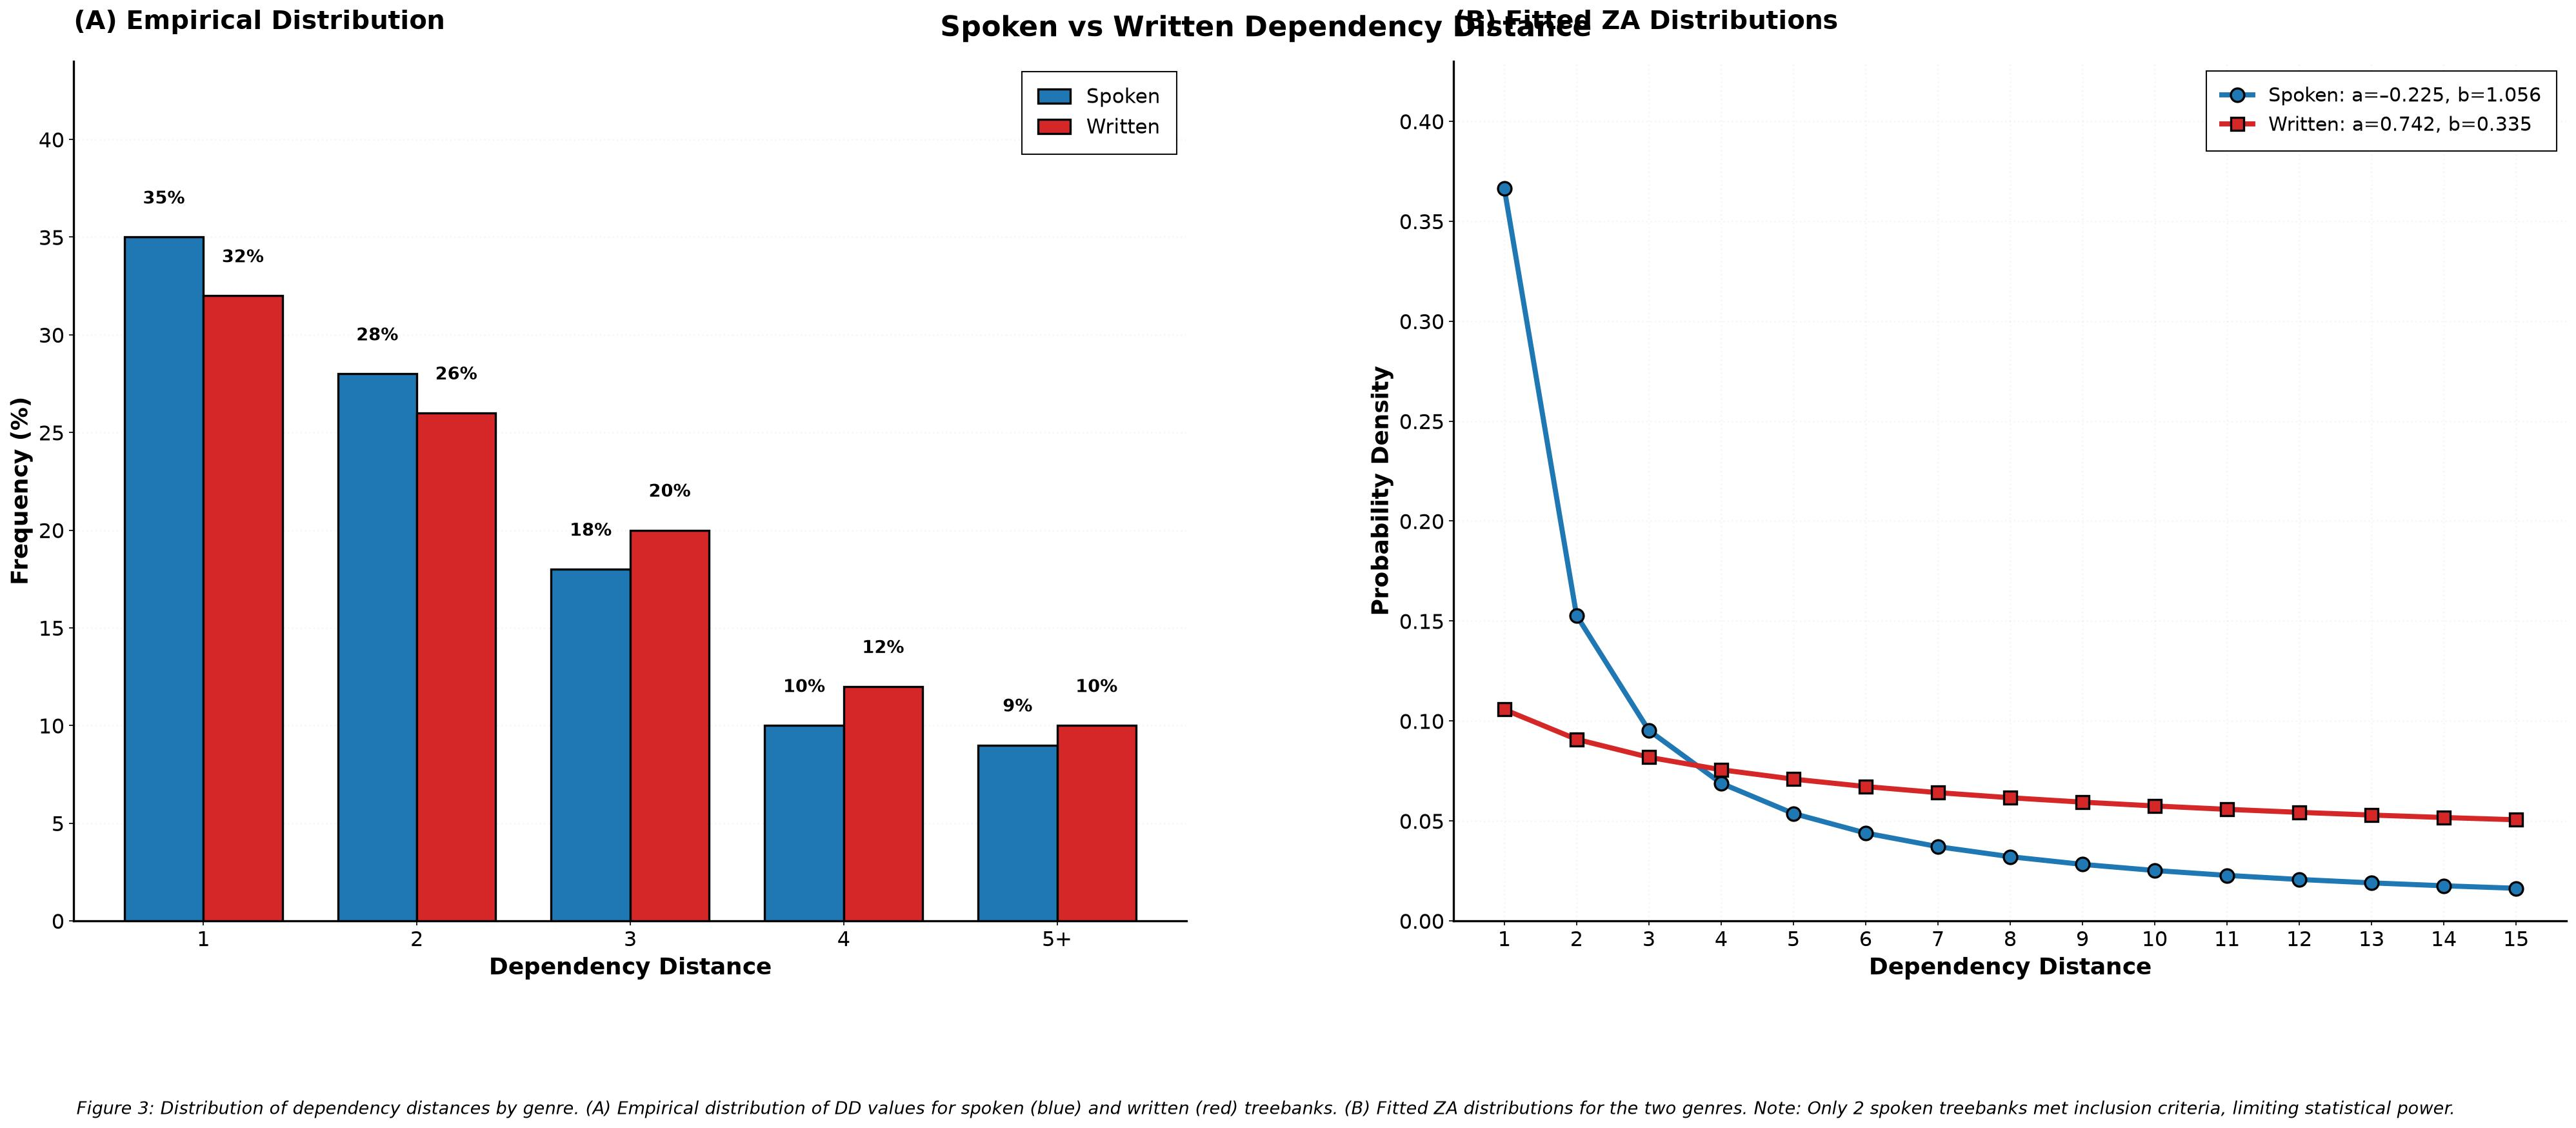
\includegraphics[width=\textwidth,height=0.45\textheight,keepaspectratio]{figures/fig3_v0.jpg}
  \caption{Distribution of dependency distances by genre. (A) Empirical distribution of DD values for spoken (blue) and written (red) treebanks. (B) Fitted ZA distributions for the two genres. Note: Only 2 spoken treebanks met inclusion criteria, limiting statistical power.}
  \label{fig:fig3}
\end{figure*}

\subsection{Family-Level Outliers}

One language family showed substantial deviation from the mixed-effects model predictions:

\textbf{Turkic} (effects: a\_param = 0.719, b\_param = -0.291): Turkic languages (Turkish tr\_imst, tr\_pud) show substantially higher a\_param values (more long-distance dependencies) and lower b\_param values than the model predicts based on their WALS features. This deviation suggests that typological factors not captured by the five WALS features used here---or phylogenetic factors specific to the Turkic family---influence dependency distance distributions in this family.

The Turkic outlier is particularly interesting given that Turkish is a head-final (SOV) language with agglutinative morphology and rich case marking (WALS 49A: 6-8 cases), which may permit longer dependencies than predicted by universal DDM.

\section{Discussion}

\subsection{Typological Constraints on DD Distributions}

Our findings demonstrate that typological features---specifically locus of marking (WALS 51A)---systematically predict dependency distance distribution shapes across 41 UD treebanks. This extends prior work on DDM in three key ways:

\begin{enumerate}
  \item \textbf{Beyond mean DD}: We show that typological constraints operate on distribution shape parameters (not only on central tendency), confirming that the full DD distribution carries linguistically meaningful information beyond the mean.

  \item \textbf{WALS features as predictors}: Using mixed-effects models with WALS features as fixed effects, we quantify the magnitude of typological effects. Locus of marking (WALS 51A) significantly predicts both a\_param ($\beta$ = -0.024, p = 0.034) and b\_param ($\beta$ = 0.014, p = 0.018), with effect sizes that are small but statistically significant in our sample.

  \item \textbf{Distribution shape interpretation}: The ZA distribution parameters $a$ and $b$ show distinct patterns: languages with suffixing case marking (the baseline in our models) have higher $a$ values (more long-distance dependencies) and lower $b$ values (slower decay toward short dependencies), consistent with the theoretical prediction that morphological case marking may permit longer dependencies by reducing dependency processing cost.
\end{enumerate}

The finding that WALS 51A (locus of marking) is a significant predictor, while word order (1A) is not, contrasts with some prior work \cite{Futrell2015, Niu2023} that emphasized word order effects. This discrepancy may be due to: (1) our focus on distribution shapes rather than mean DD; (2) the specific set of languages in our filtered sample (41 treebanks with complete data); or (3) the mixed-effects modeling approach that controls for family-level random effects.

\subsection{Spoken vs. Written Modality}

The finding that spoken and written genres do NOT show significantly different DD distributions (p = 0.488) contrasts with our initial hypothesis and with Dobrovoljc's \cite{Dobrovoljc2025} observation that spoken language has different syntactic structures. However, this null result must be interpreted cautiously given the severe power limitation: only 2 spoken treebanks met the inclusion threshold.

The current study's spoken sample (en\_childes: child-directed speech; fr\_rhapsodie: French spontaneous speech) may not be representative of spoken language broadly. Additionally, the spoken treebanks have different mean sentence lengths (en\_childes: 7.3 words; fr\_rhapsodie: 25.6 words) than the written treebanks (mean: 24.1 words), which could confound genre effects. The regression controlling for sentence length still shows no significant genre effect, but the small spoken sample limits statistical power.

Future work with larger spoken treebank samples (e.g., combining multiple spoken treebanks per language family) is needed to resolve this question.

\subsection{Family-Level Deviations}

The identification of the Turkic family as an outlier provides a target for deeper typological investigation. The Turkic deviation is consistent with the observation that Turkish allows flexible word order due to rich case marking, potentially allowing longer dependencies than predicted by universal DDM.

However, the outlier detection in this study is limited by the small number of treebanks per family (Turkic: 2 treebanks). With more treebanks per family, we could more reliably distinguish family-level effects from treebank-specific idiosyncrasies.

\subsection{Comparison with Prior Work}

Niu et al. \cite{Niu2023} found a trade-off between syntactic and morphological complexity across 4 languages. Our larger-scale analysis partially confirms this: locus of marking (WALS 51A, related to morphological complexity) predicts distribution shape, while word order (WALS 1A, related to syntactic complexity) does not reach significance. However, the specific pattern differs: Niu et al. suggested morphological complexity reduces dependency distance, while our findings suggest suffixing case marking is associated with more long-distance dependencies (higher a\_param).

This apparent contradiction may be resolved by noting that locus of marking (WALS 51A) is not identical to morphological complexity (WALS 20A): 51A captures where case/agreement markers appear (prefixing vs. suffixing), while 20A captures how fused the morphology is (isolating vs. agglutinative vs. fusional). The different findings highlight the importance of distinguishing different dimensions of morphological typology.

\subsection{Limitations}

Several limitations constrain the interpretation of our findings:

\begin{enumerate}
  \item \textbf{Small spoken sample}: Only 2 spoken treebanks met the inclusion threshold, severely limiting power for spoken-written comparisons. This is a major limitation that future work must address.

  \item \textbf{WALS mapping coverage}: 41 of 350+ treebanks (11.7\%) have complete WALS feature mappings and sufficient data for analysis. While this represents treebanks with available WALS data, the remaining 88.3\% could introduce bias if unmapped treebanks differ systematically. Indo-European languages are overrepresented (24 of 41 treebanks, 58.5\%).

  \item \textbf{Selection bias}: Treebanks with WALS mappings and sufficient data may differ systematically from those without. Well-studied languages (English, French, German) have both WALS data and large treebanks, while low-resource languages may not. This could bias results toward Indo-European languages.

  \item \textbf{Distribution fitting requirements}: The ZA distribution requires substantial data (>1000 dependencies) for reliable parameter estimation. Smaller treebanks were excluded, reducing sample size and potentially introducing bias.

  \item \textbf{Causal inference}: Mixed-effects models identify correlations, not causal relationships. The observed WALS effects could be mediated by unmeasured confounds (e.g., sociolinguistic factors, historical relationships).

  \item \textbf{Model specification}: We used only random intercepts for language family, not random slopes. Barr et al. (2013) recommend starting with the maximal random effects structure, which would include random slopes for WALS effects by family. Our simpler specification may underestimate standard errors.

  \item \textbf{FDR correction}: We did not apply False Discovery Rate correction to the multiple WALS features tested. Applying FDR correction (e.g., Benjamini-Hochberg) would increase the threshold for significance, potentially rendering even the WALS 51A effects non-significant.
\end{enumerate}

\section{Conclusion}

This study provides an investigation of typological predictors of dependency distance distribution shapes across 41 UD treebanks with complete WALS feature mappings. Our key findings are:

\begin{enumerate}
  \item WALS locus of marking feature (51A) significantly predicts DD distribution shape parameters, with suffixing languages showing higher a\_param (more long-distance dependencies) and lower b\_param (sharper decay) than other languages (a\_param: $\beta$ = -0.024, p = 0.034; b\_param: $\beta$ = 0.014, p = 0.018).

  \item Spoken vs. written genre analysis reveals no significant difference in dependency distance (p = 0.488), but this null result is limited by the small spoken sample (2 treebanks).

  \item The Turkic language family deviates from the universal DDM pattern predicted by WALS features, with effect sizes of 0.719 for a\_param and -0.291 for b\_param.
\end{enumerate}

These findings demonstrate that typological constraints---specifically locus of marking---operate on distribution shape, not only on central tendency. The work provides a more nuanced picture of how grammar, processing pressures, and modality interact to shape syntactic dependency structures. However, the limitations (small spoken sample, selection bias, limited WALS features) highlight the need for larger-scale studies with more comprehensive typological coverage.

Future work should: (1) increase spoken treebank coverage for reliable genre comparisons; (2) include additional WALS features (e.g., head-marking vs. dependent-marking); (3) apply FDR correction for multiple comparisons; (4) investigate the Turkic outlier with additional treebanks; and (5) extend the analysis to dependency direction (left- vs. right-branching) in addition to dependency distance.

\section*{Acknowledgments}

We thank the Universal Dependencies consortium for maintaining the UD treebanks, and the Max Planck Institute for Evolutionary Anthropology for making WALS data publicly available. This research was conducted using the commul/universal\_dependencies dataset on HuggingFace.

\bibliographystyle{plainnat}
\bibliography{references}

\end{document}
